% =======================================================================
% APPENDIX A: Data Construction and Supplementary Evidence
% =======================================================================

\clearpage
\section{Appendix A: Data Construction }
\label{app:A}

This appendix documents the construction of the main variables, clarifies the harmonisation of demographic categories across datasets, and reports supplementary robustness evidence that supports the interpretation of the main results. The purpose is not to introduce a separate empirical design, but to make the preferred design more transparent and reproducible.

% -----------------------------------------------------------------------
\subsection{Data construction and harmonisation}
\label{app:data_construction}

The analysis combines three sources aggregated to the microregion-year level: ProUni administrative records, RAIS formal labour-market data, and the 2010 Demographic Census. ProUni records are used to construct scholarship exposure, RAIS is used to measure formal-sector labour-market outcomes, and the Census provides baseline population denominators and demographic composition.

The treatment variable is cumulative ProUni scholarship intensity measured relative to the local youth population. In the baseline design, exposure is lagged to reflect the time required for higher-education participation to affect early-career labour-market outcomes.

Outcome variables are constructed from RAIS for workers in the early-career age range used in the main text. Because RAIS covers formal employment only, employment effects should be interpreted as formal-sector extensive-margin effects rather than as complete labour-market quantity effects.

Demographic heterogeneity is analysed using harmonised gender and ethnicity categories. Following the main analysis, workers recorded in the IBGE categories \textit{Parda} and \textit{Preta} are grouped into a single non-white category for the ethnicity heterogeneity exercises, while observations with missing ethnicity are excluded from those subgroup specifications.

\begin{table}[H]
\centering
\caption{Principal administrative codes used in variable construction}
\label{tab:key_codes_script}
\begin{tabular}{p{2.5cm} p{3.6cm} p{2.3cm} p{6.6cm}}
\toprule
\textbf{Source} & \textbf{Variable} & \textbf{Key codes} & \textbf{Role in the script} \\
\midrule
RAIS & \texttt{tipo\_vinculo} & 10 = CLT & Restricts the sample to formal private-sector employment relationships. \\
RAIS & \texttt{vinculo\_ativo\_3112} & 1 = active on 31 Dec. & Keeps only active employment links at year-end. \\
RAIS & \texttt{sexo} & 1 = male; 2 = female & Defines gender-specific heterogeneity subsamples. \\
RAIS & \texttt{raca\_cor} & 1 = Indigenous; 2 = White; 4 = Black; 8 = Parda & White is coded as 2; the non-white group is defined as 1, 4, and 8. \\
RAIS & \texttt{grau\_instrucao\_apos\_2005} & 9 = completed tertiary; 10 = master's; 11 = doctorate & Used to construct the college-share first stage for the Wald/LATE exercise. \\
ProUni & \texttt{sexo} & 1 = female; 2 = male & Descriptive composition of scholarship recipients. \\
ProUni & \texttt{raca\_cor} & administrative ethnicity/colour codes & Descriptive composition of scholarship recipients. \\
ProUni & \texttt{tipo\_bolsa} & 1 = full; 2 = partial 50\%; 3 = complementary 25\% & Describes scholarship type in the ProUni microdata. \\
Census 2010 & \texttt{v6036} & age in years & Restricts the denominator to the population aged 18--24. \\
Census 2010 & \texttt{peso\_amostral} & survey weight & Expands observations to the microregion youth population. \\
Census 2010 & \texttt{v0601} & 1 = male; 2 = female & Baseline demographic composition. \\
Census 2010 & \texttt{v0606} & 1 = White; 2 = Black; 3 = Asian descent; 4 = Parda; 5 = Indigenous & Baseline ethnicity composition and non-white denominator construction. \\
Census 2010 & \texttt{v6400}, \texttt{v0633}, \texttt{v6511}, \texttt{v6532}, \texttt{v0627}, \texttt{v0628}, \texttt{v0616} & see IBGE dictionary & Used to build pre-treatment covariates for the doubly robust specification. \\
\bottomrule
\end{tabular}
\caption*{\footnotesize \textit{Notes:} The table reports only the codes that directly affect sample restrictions, subgroup definitions, treatment construction, or pre-treatment covariates in the empirical script. Full official dictionaries downloaded from Base dos Dados are provided separately in the documentation files.}
\end{table}


To support reproducibility, the underlying variable dictionaries and audit files are stored in the project repository:
\begin{itemize}
    \item \texttt{Documentation/appendix\_prouni\_codes.csv}
    \item \texttt{Documentation/appendix\_rais\_codes.csv}
    \item \texttt{Documentation/appendix\_census\_codes.csv}
    \item \texttt{Documentation/audit\_log.rds}
\end{itemize}

These files contain the raw keys, category mappings, and processing notes used to construct the analytical sample and its main subgroup definitions.

% -----------------------------------------------------------------------
\subsection{Supplementary summary estimates}
\label{app:summary_estimates}

Table~\ref{tab:att_master} reports the consolidated ATT estimates across the principal specifications discussed in the main text, including pooled wage effects, employment effects, heterogeneity estimates, cohort decompositions, and benchmark TWFE results.

% latex table generated in R 4.5.1 by xtable 1.8-4 package
% Fri Mar  6 00:30:52 2026
\begin{table}[ht]
\centering
\begin{tabular}{lrrrrr}
  \toprule
Model & ATT_display & SE_display & t_stat & Pretrend_p & N_obs \\ 
  \midrule
Low/Wages & +0.0128 & (0.0128) & 1.00 & 0.359 & 3906 \\ 
  High/Wages & -0.0070 & (0.0074) & -0.95 & 0.915 & 3528 \\ 
  Marginal/Wages & +0.0136* & (0.0078) & 1.74 & 0.362 & 3752 \\ 
  Low/Emp & +0.0182 & (0.0332) & 0.55 & 0.120 & 3906 \\ 
  High/Emp & +0.0065 & (0.0396) & 0.16 & 0.809 & 3528 \\ 
  Marginal/Emp & -0.0386 & (0.0335) & -1.15 & 0.597 & 3752 \\ 
  Male/Low & +0.0167 & (0.0169) & 0.99 & 0.418 & 3906 \\ 
  Female/Low & -0.0003 & (0.0007) & -0.43 & 0.953 & 3905 \\ 
  Male/High & -0.0083 & (0.0092) & -0.90 & 0.918 & 3528 \\ 
  Female/High & -0.0041 & (0.0073) & -0.56 & 0.736 & 3527 \\ 
  White/Low & -0.0022 & (0.0088) & -0.25 & 0.355 & 3903 \\ 
  Nonwhite/Low & +0.0128 & (0.0119) & 1.08 & 0.405 & 3906 \\ 
  White/High & -0.0048 & (0.0088) & -0.55 & 0.683 & 3525 \\ 
  Nonwhite/High & -0.0070 & (0.0071) & -0.99 & 0.916 & 3528 \\ 
  Low/Lag3 & -0.0001 & (0.0076) & -0.01 & 0.373 & 3906 \\ 
  High/Lag3 & -0.0019 & (0.0059) & -0.32 & 0.099 & 3528 \\ 
  Low/DR & +0.0259* & (0.0145) & 1.79 & 0.535 & 3906 \\ 
  Low/q25_75 & +0.0015 & (0.0126) & 0.12 & 0.097 & 3906 \\ 
  High/q25_75 & -0.0051 & (0.0095) & -0.54 & 0.213 & 3920 \\ 
  Low/q33_67 & +0.0089 & (0.0124) & 0.72 & 0.860 & 3906 \\ 
  High/q33_67 & -0.0078 & (0.0062) & -1.26 & 0.234 & 5208 \\ 
  Gap/Low & -0.0054 & (0.0120) & -0.45 & 0.707 & 3904 \\ 
  Gap/High & +0.0234 & (0.0273) & 0.86 & 0.539 & 3526 \\ 
  Young/Low & +0.0095 & (0.0107) & 0.89 & 0.644 & 3906 \\ 
  Young/High & -0.0042 & (0.0132) & -0.32 & 0.162 & 3528 \\ 
  Old/Low & +0.0149 & (0.0125) & 1.19 & 0.871 & 3904 \\ 
  Old/High & -0.0276 & (0.0199) & -1.39 & 0.981 & 3526 \\ 
  CollegeGap/Low & -0.0003 & (0.0028) & -0.11 & 0.924 & 3904 \\ 
  CollegeGap/High & +0.0024 & (0.0031) & 0.77 & 0.124 & 3526 \\ 
  WageGap/Male/Low & -0.0066 & (0.0159) & -0.42 & 0.521 & 3899 \\ 
  WageGap/Male/High & +0.0315 & (0.0325) & 0.97 & 0.605 & 3521 \\ 
  WageGap/Female/Low & -0.0030 & (0.0024) & -1.25 & 0.595 & 3897 \\ 
  WageGap/Female/High & +0.0175 & (0.0193) & 0.91 & 0.702 & 3520 \\ 
  WageGap/White/Low & +0.0135 & (0.0141) & 0.96 & 0.547 & 3898 \\ 
  WageGap/White/High & -0.0252** & (0.0103) & -2.45 & 0.851 & 3520 \\ 
  WageGap/Nonwhite/Low & -0.0054 & (0.0113) & -0.48 & 0.730 & 3904 \\ 
  WageGap/Nonwhite/High & +0.0234 & (0.0276) & 0.85 & 0.531 & 3526 \\ 
  BC_Gap/Low & +0.0116 & (0.0092) & 1.26 & 0.522 & 3069 \\ 
  BC_Gap/High & +0.0018 & (0.0130) & 0.14 & 0.823 & 2772 \\ 
  BC_Exposed/Low & +0.0107 & (0.0111) & 0.96 & 0.967 & 3896 \\ 
  BC_Control/Low & -0.0009 & (0.0094) & -0.10 & 0.904 & 3906 \\ 
  TWFE/Wages & -0.0065* & (0.0037) & -1.76 &  & 7812 \\ 
  TWFE/Employment & -0.0467*** & (0.0180) & -2.59 &  & 7812 \\ 
   \bottomrule
\end{tabular}
\caption{Summary of ATT Estimates Across All Specifications} 
\label{tab:att_master}
\end{table}


Table~\ref{tab:att_master} should be read as a compact summary of the broader empirical pattern rather than as a menu of equally preferred specifications. The preferred interpretation remains anchored in the staggered-adoption event-study design reported in the main chapter.

% -----------------------------------------------------------------------
\subsection{Robustness to alternative specifications}
\label{app:robustness}

Table~\ref{tab:robustness} reports the main robustness checks. These include the baseline wage specifications, a three-year lag alternative, a doubly robust estimator, and alternative treatment-intensity partitions based on the 25/75 and 33/67 percentiles.

% latex table generated in R 4.5.1 by xtable 1.8-4 package
% Fri Mar  6 00:30:53 2026
\begin{table}[ht]
\centering
\begin{tabular}{lrrrrrr}
  \toprule
Model & ATT & SE & t\_stat & Pretrend\_p & N\_treated & N\_notyet \\ 
  \midrule
Low/Wages & 0.0128 & 0.0128 & 1.00 & 0.359 & 167 & 112 \\ 
  High/Wages & -0.0070 & 0.0074 & -0.95 & 0.915 & 140 & 112 \\ 
  Low/Lag3 & -0.0001 & 0.0076 & -0.01 & 0.373 & 167 & 112 \\ 
  High/Lag3 & -0.0019 & 0.0059 & -0.32 & 0.099 & 140 & 112 \\ 
  Low/DR & 0.0259 & 0.0145 & 1.79 & 0.535 & 167 & 112 \\ 
  Low/q25\_75 & 0.0015 & 0.0126 & 0.12 & 0.097 & 139 & 140 \\ 
  High/q25\_75 & -0.0051 & 0.0095 & -0.54 & 0.213 & 140 & 140 \\ 
  Low/q33\_67 & 0.0089 & 0.0124 & 0.72 & 0.860 & 93 & 186 \\ 
  High/q33\_67 & -0.0078 & 0.0062 & -1.26 & 0.234 & 186 & 186 \\ 
   \bottomrule
\end{tabular}
\caption{Robustness: Alternative Specifications and Cutoffs} 
\label{tab:robustness}
\end{table}


Across these specifications, the qualitative contrast between low- and high-exposure markets is broadly preserved. At the same time, the magnitude and statistical precision of the low-dose wage effect vary across estimator and cutoff choices, so the robustness evidence is supportive but not uniform. For this reason, the thesis interprets the low-dose wage gains as suggestive reduced-form evidence rather than as definitive proof of a stable structural effect.

% -----------------------------------------------------------------------
\subsection{Supplementary robustness figures}
\label{app:robustness_figures}

Figure~\ref{fig:app_altcut} reports the event-study estimates under alternative treatment-intensity cutoffs. The figure is useful for assessing whether the baseline low-versus-high comparison is driven mechanically by the chosen discretisation rule.

\begin{figure}[H]
    \centering
    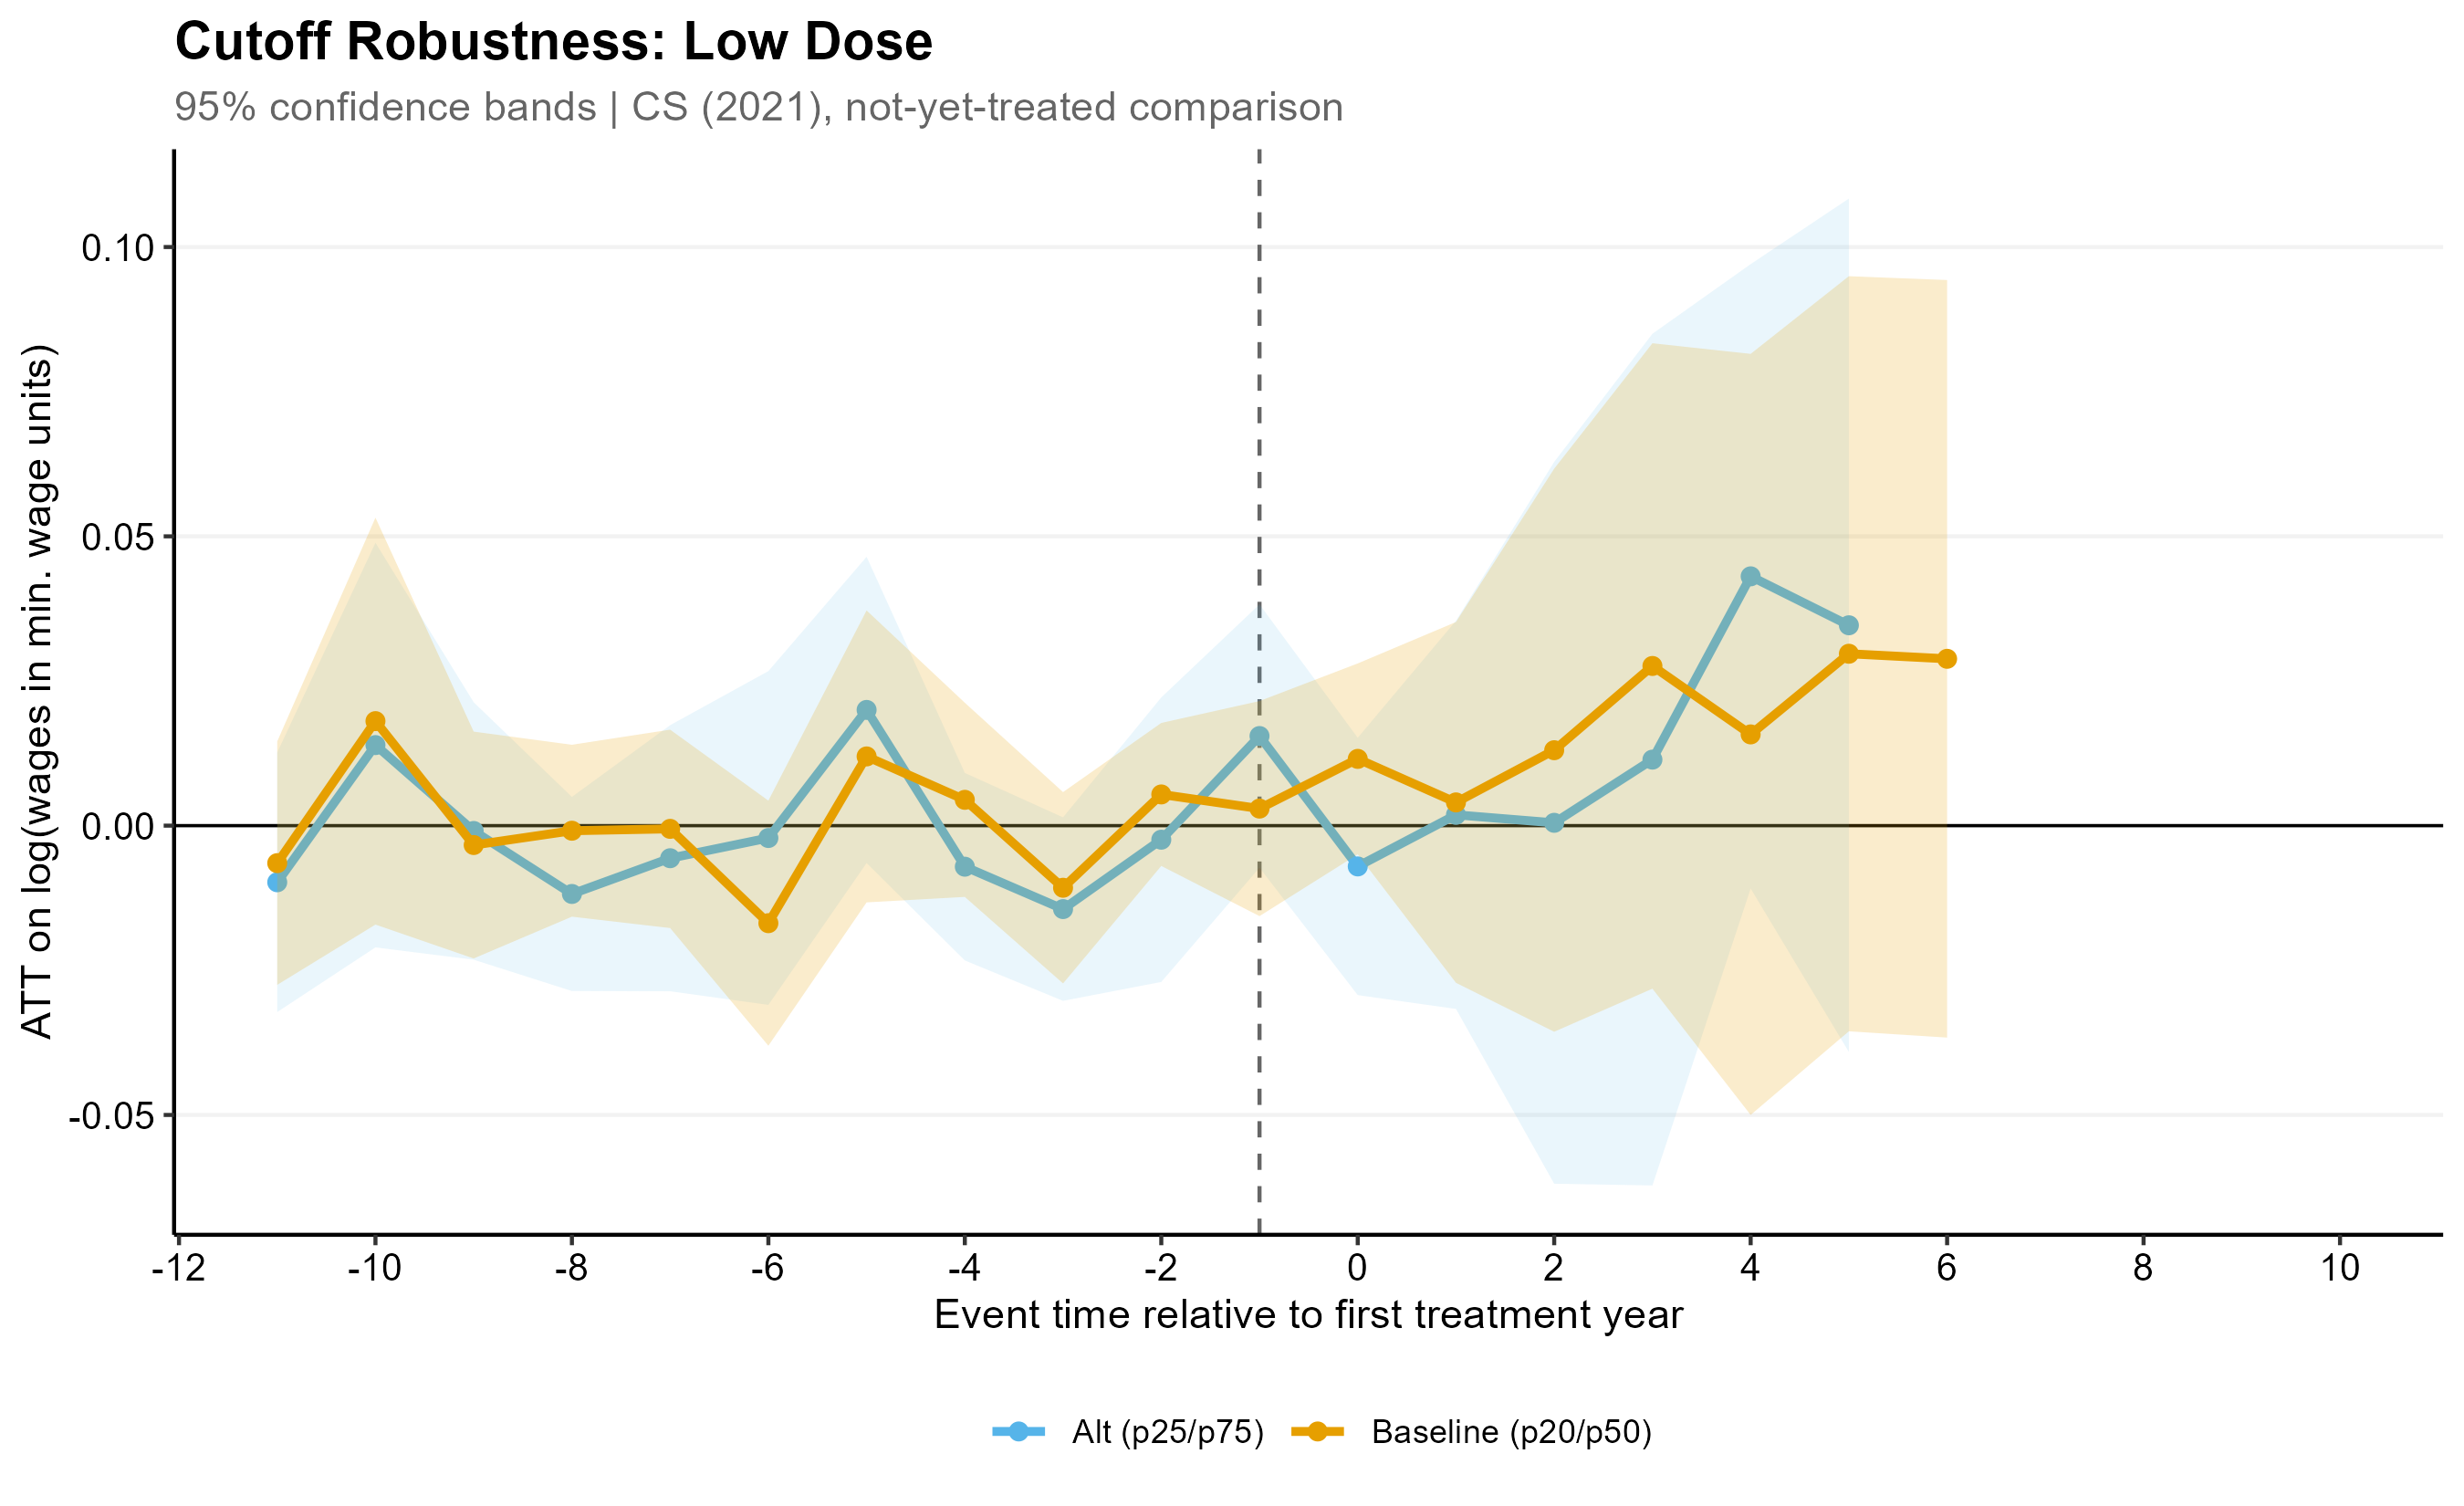
\includegraphics[width=0.84\textwidth]{Figures/fig_9_altcut_low.png}
    \caption{\textbf{Alternative dose-cutoff robustness.} Event-study estimates using alternative treatment-intensity partitions.}
    \label{fig:app_altcut}
    \caption*{\footnotesize \textit{Notes:} This figure supplements the baseline discretised design by showing how the estimated dynamics change under alternative cutoff rules. The qualitative pattern is broadly similar to the main specification, but the magnitude and precision of the low-dose estimates are sensitive to the partition used.}
\end{figure}

Figure~\ref{fig:app_lag3} evaluates the sensitivity of the results to an alternative three-year lag structure. This addresses the possibility that some beneficiaries enter the labour market faster than implied by the baseline lag.

\begin{figure}[H]
    \centering
    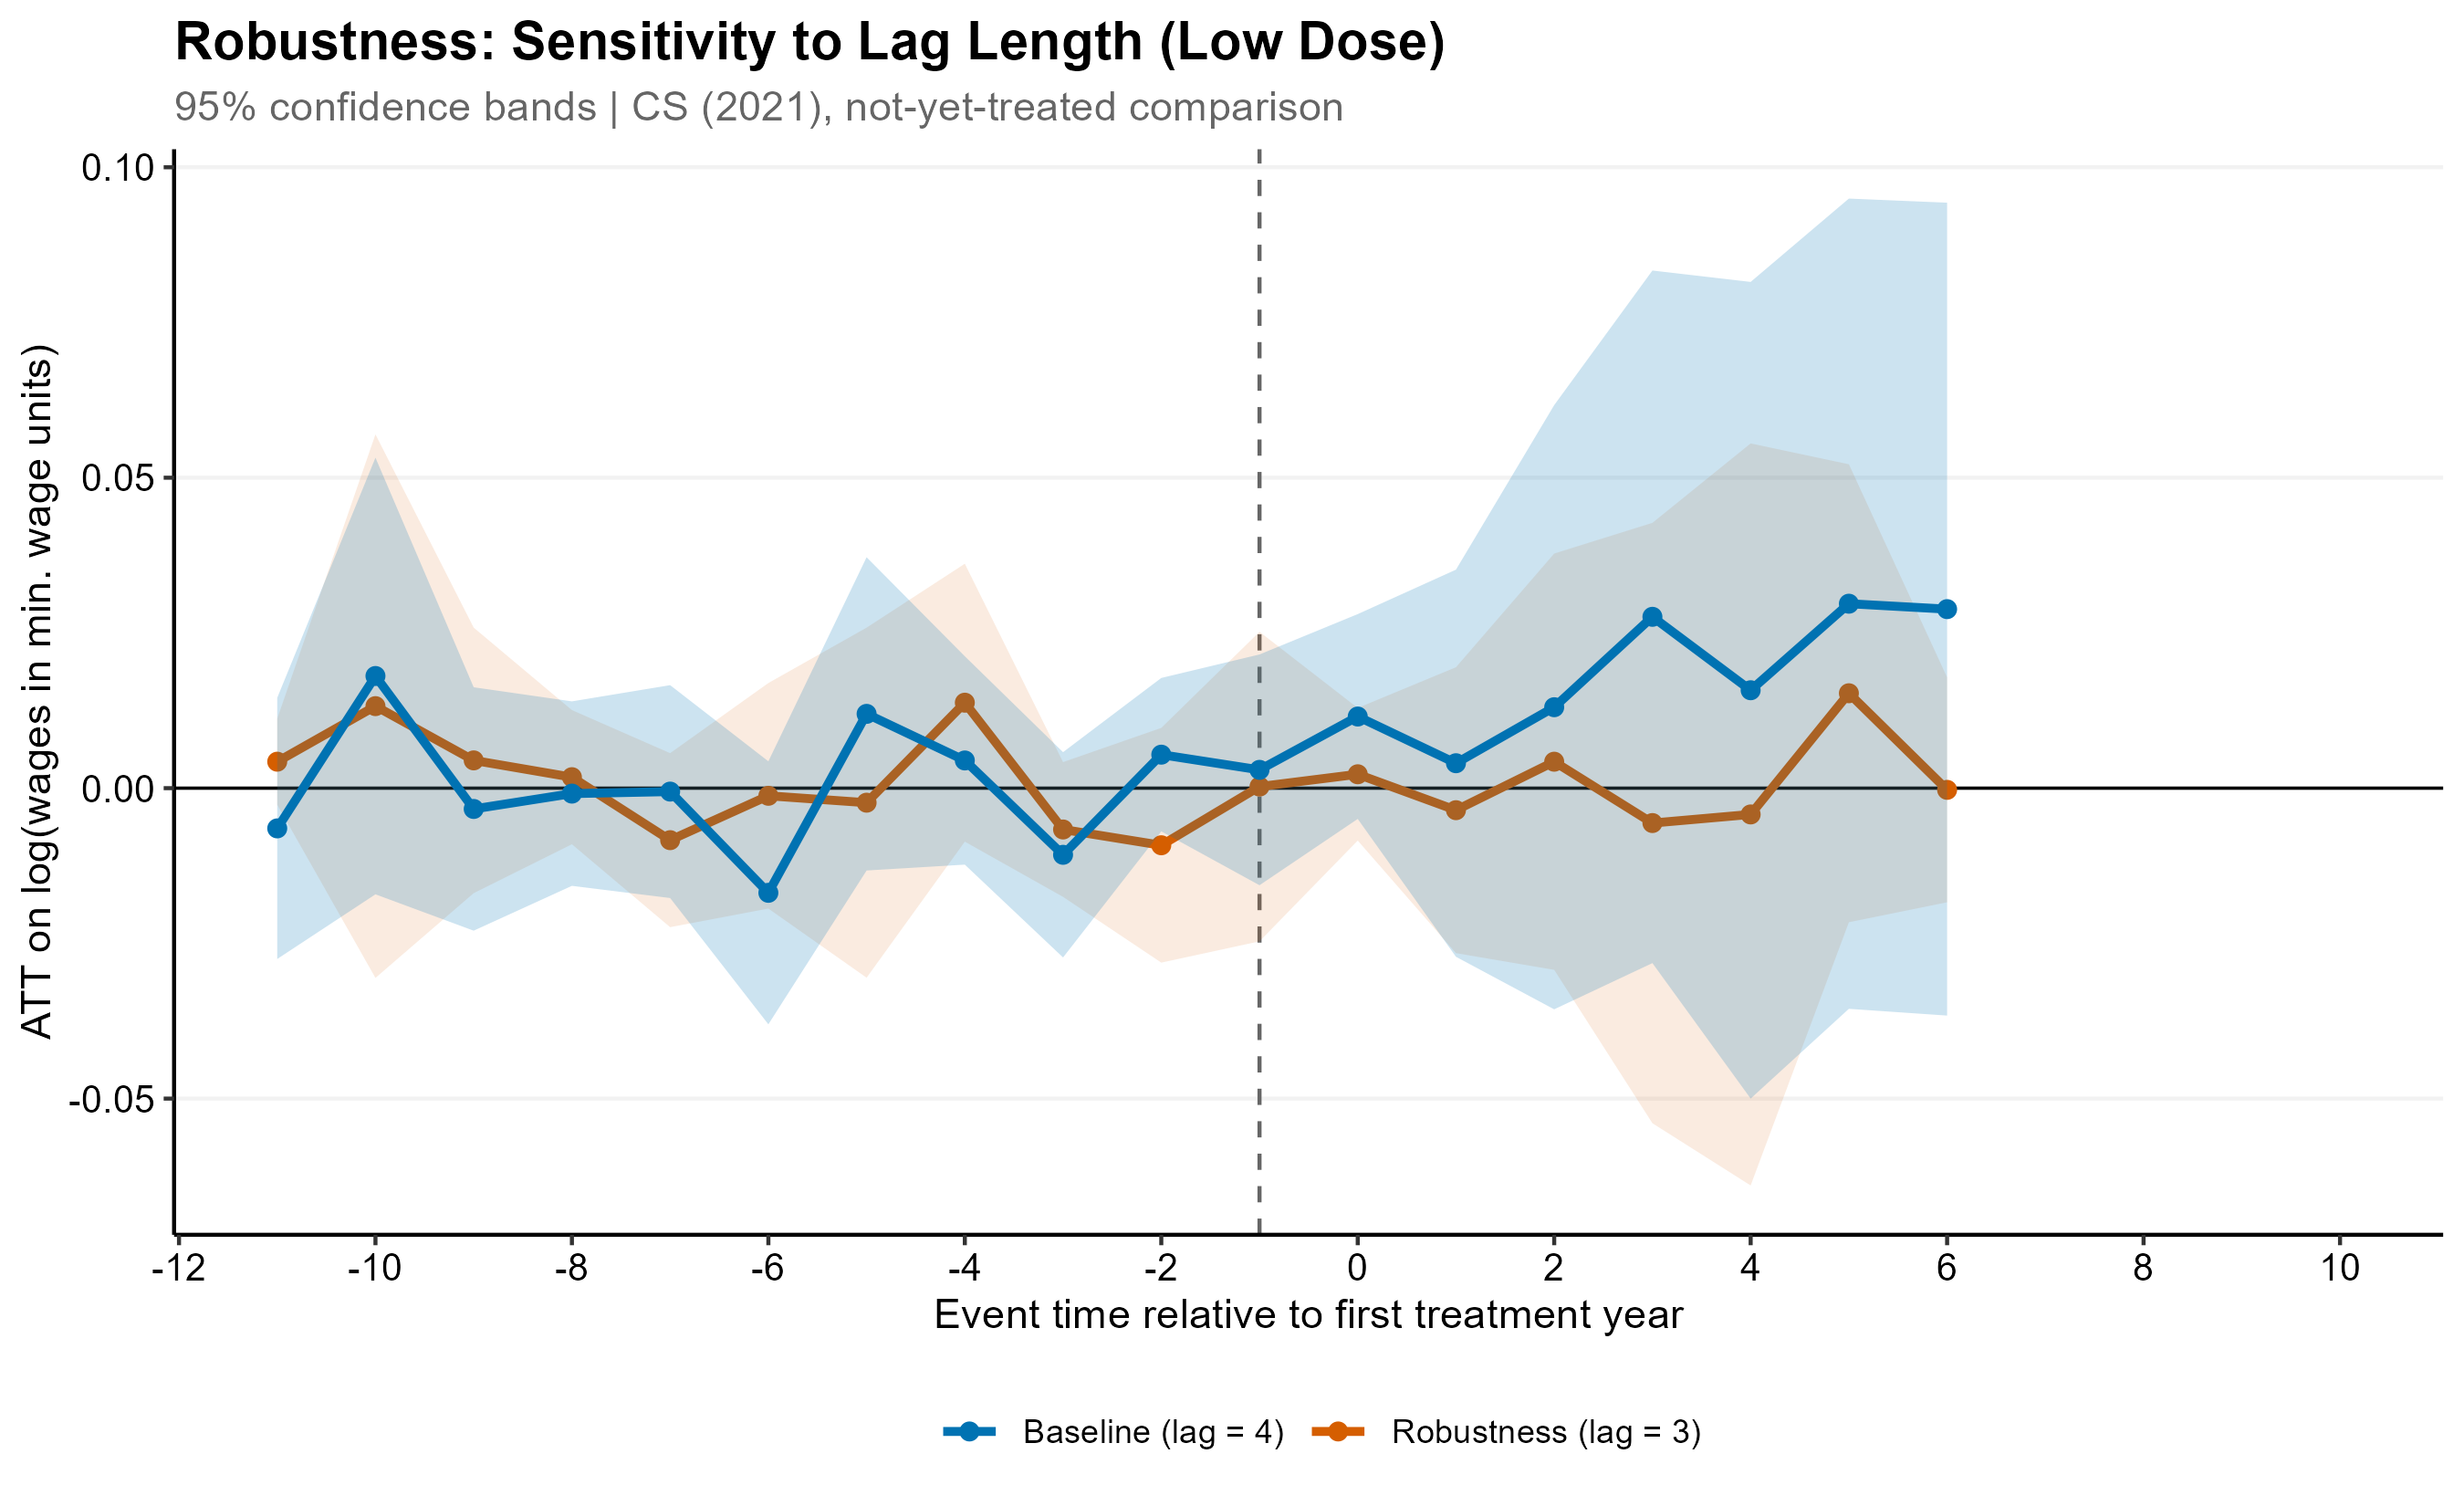
\includegraphics[width=0.84\textwidth]{Figures/fig_6_robustness_lag.png}
    \caption{\textbf{Lag sensitivity.} Event-study estimates under an alternative three-year lag.}
    \label{fig:app_lag3}
    \caption*{\footnotesize \textit{Notes:} The baseline specification uses a longer lag between scholarship allocation and labour-market exposure. This figure shows that changing the lag structure affects the estimated magnitude, which reinforces the need for cautious interpretation of the dynamic treatment effects.}
\end{figure}

Figure~\ref{fig:app_dr} reports the doubly robust version of the low-dose wage event study. This specification is informative because it checks whether the positive low-dose pattern is driven purely by unadjusted compositional differences.

\begin{figure}[H]
    \centering
    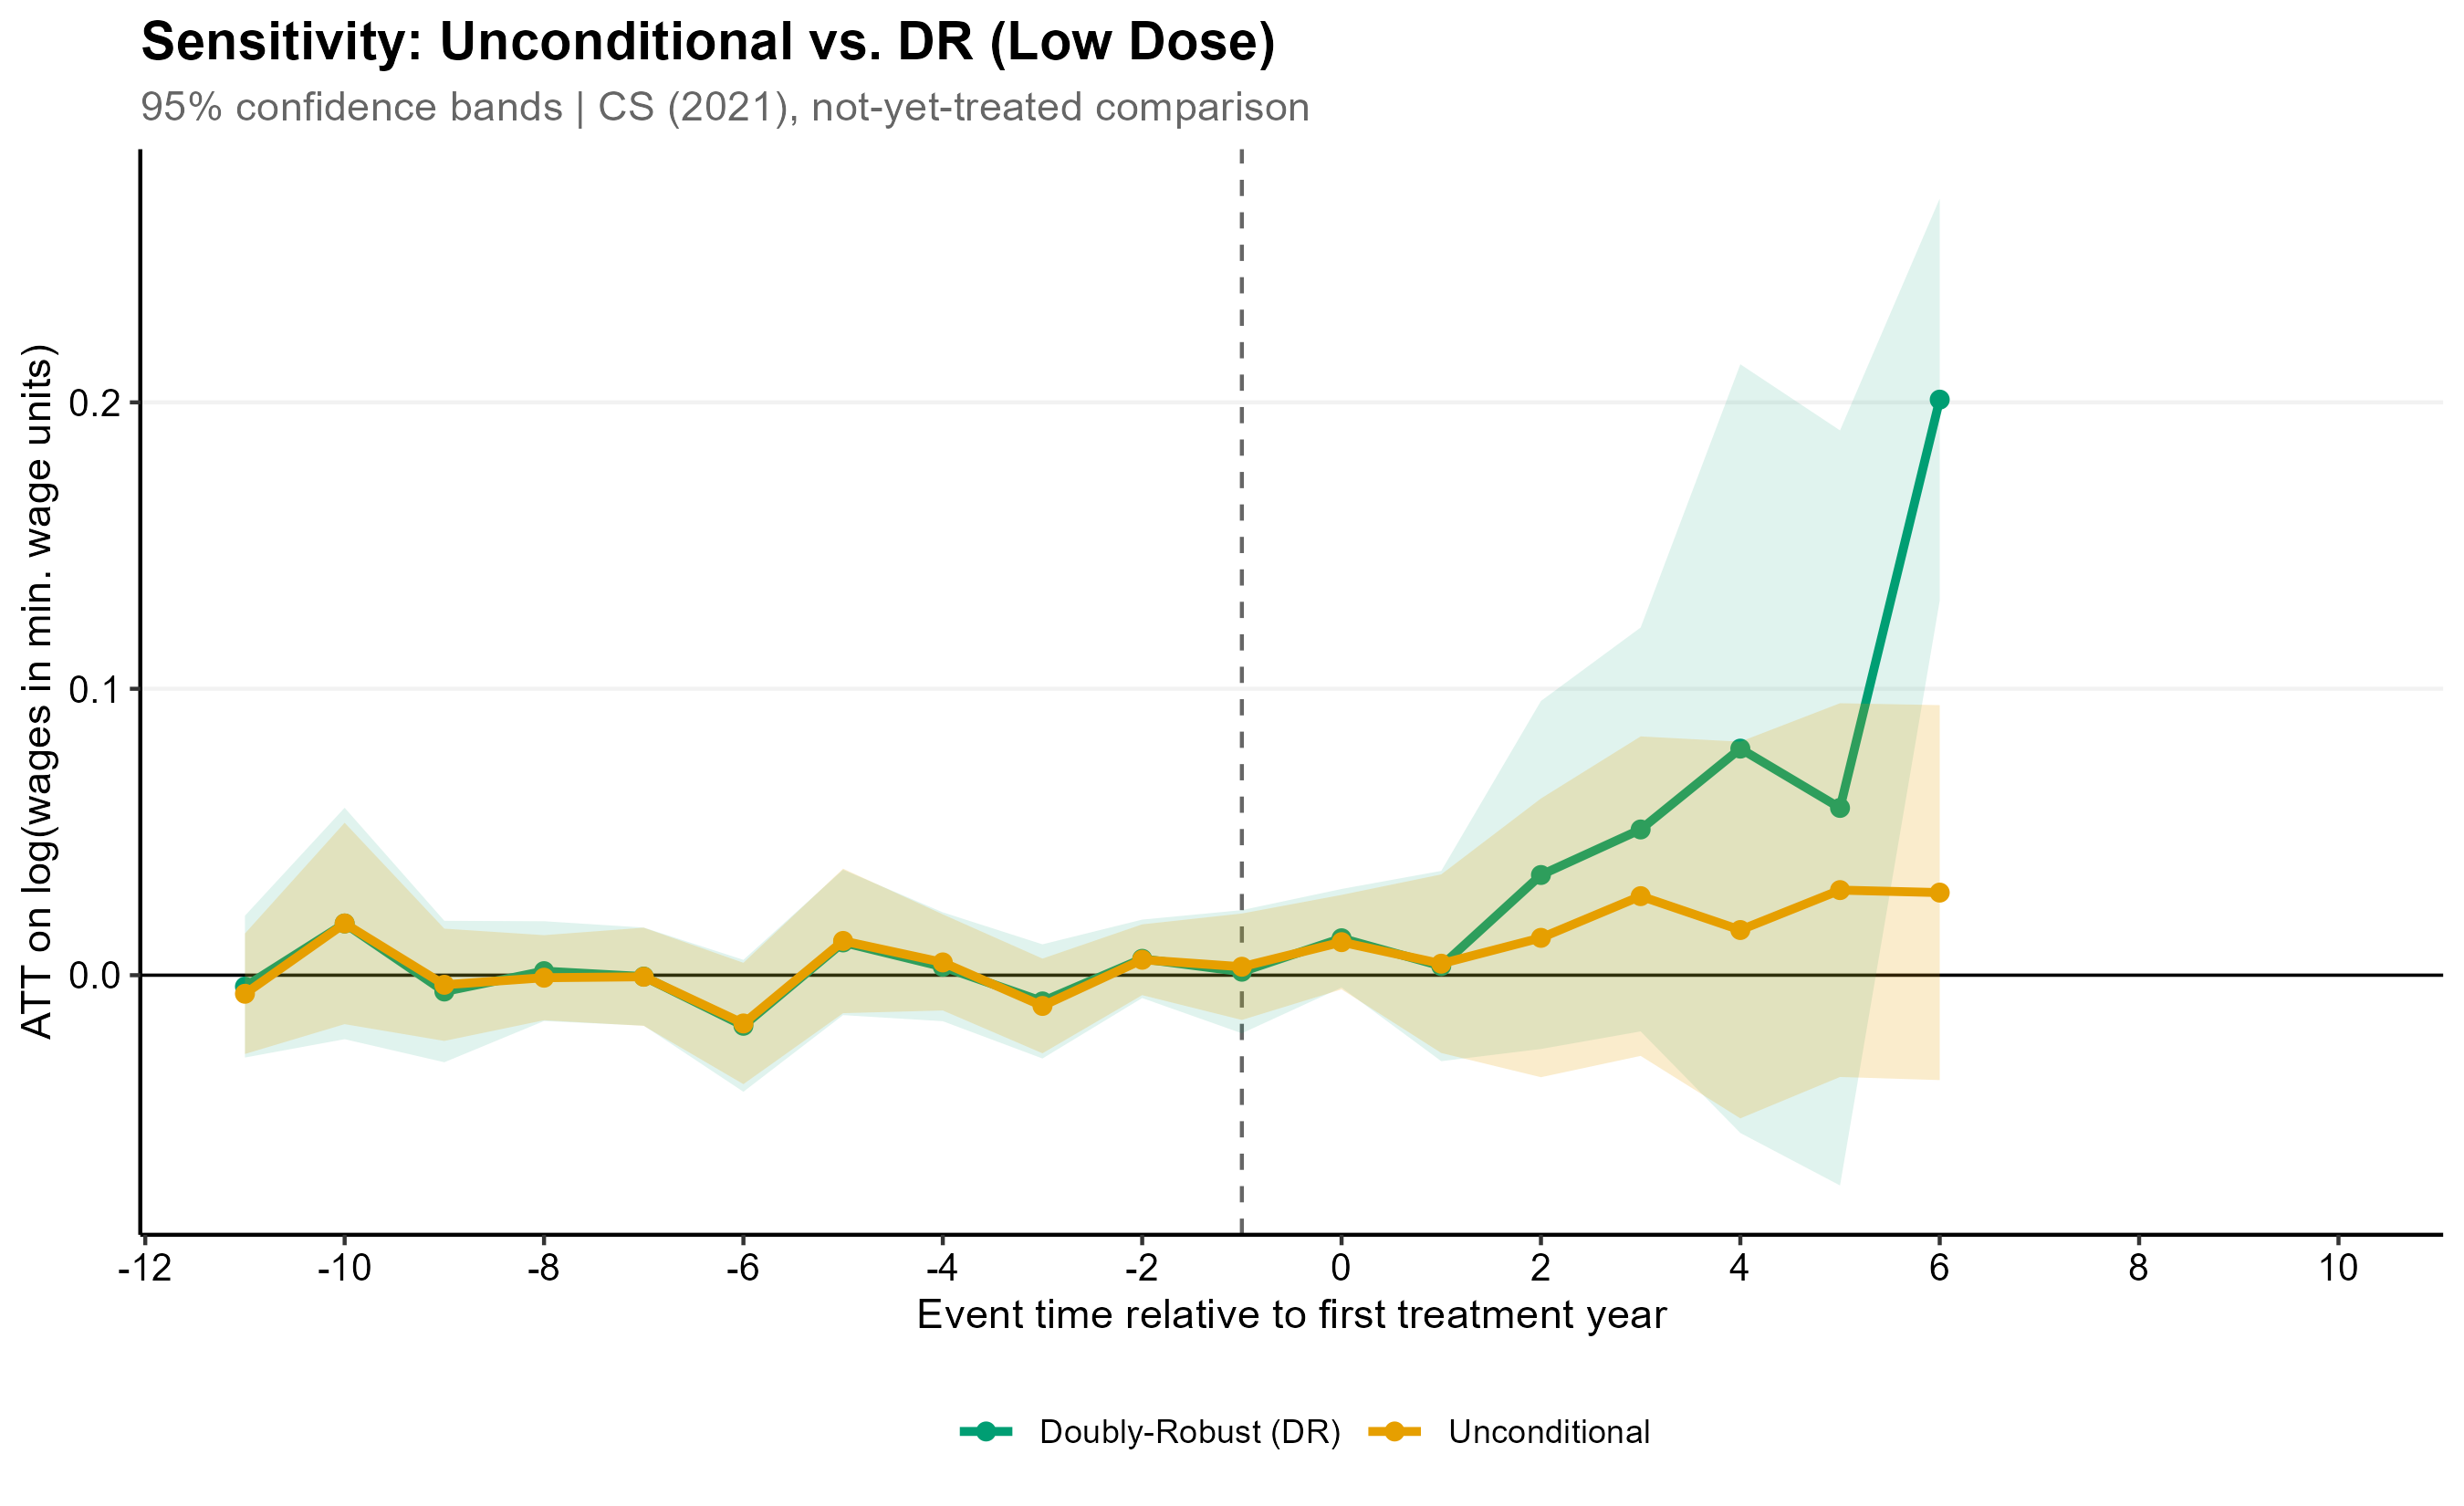
\includegraphics[width=0.84\textwidth]{Figures/fig_7_dr_low.png}
    \caption{\textbf{Doubly robust low-dose event study.} Wage effects under the doubly robust estimator.}
    \label{fig:app_dr}
    \caption*{\footnotesize \textit{Notes:} The doubly robust specification yields a larger positive point estimate than the simple baseline specification, but precision remains limited. It is therefore more appropriate to interpret this figure as supportive robustness evidence than as a separate headline result.}
\end{figure}

% -----------------------------------------------------------------------
\subsection{Additional cohort and heterogeneity evidence}
\label{app:cohort_het_appendix}

The main text reports cohort decompositions and subgroup heterogeneity because these results are useful for discussing mechanisms and distributional incidence. The supplementary figures below are included to improve transparency, but they should be interpreted with greater caution than the baseline pooled event studies because they are noisier and more sensitive to sample splitting.

\begin{figure}[H]
    \centering
    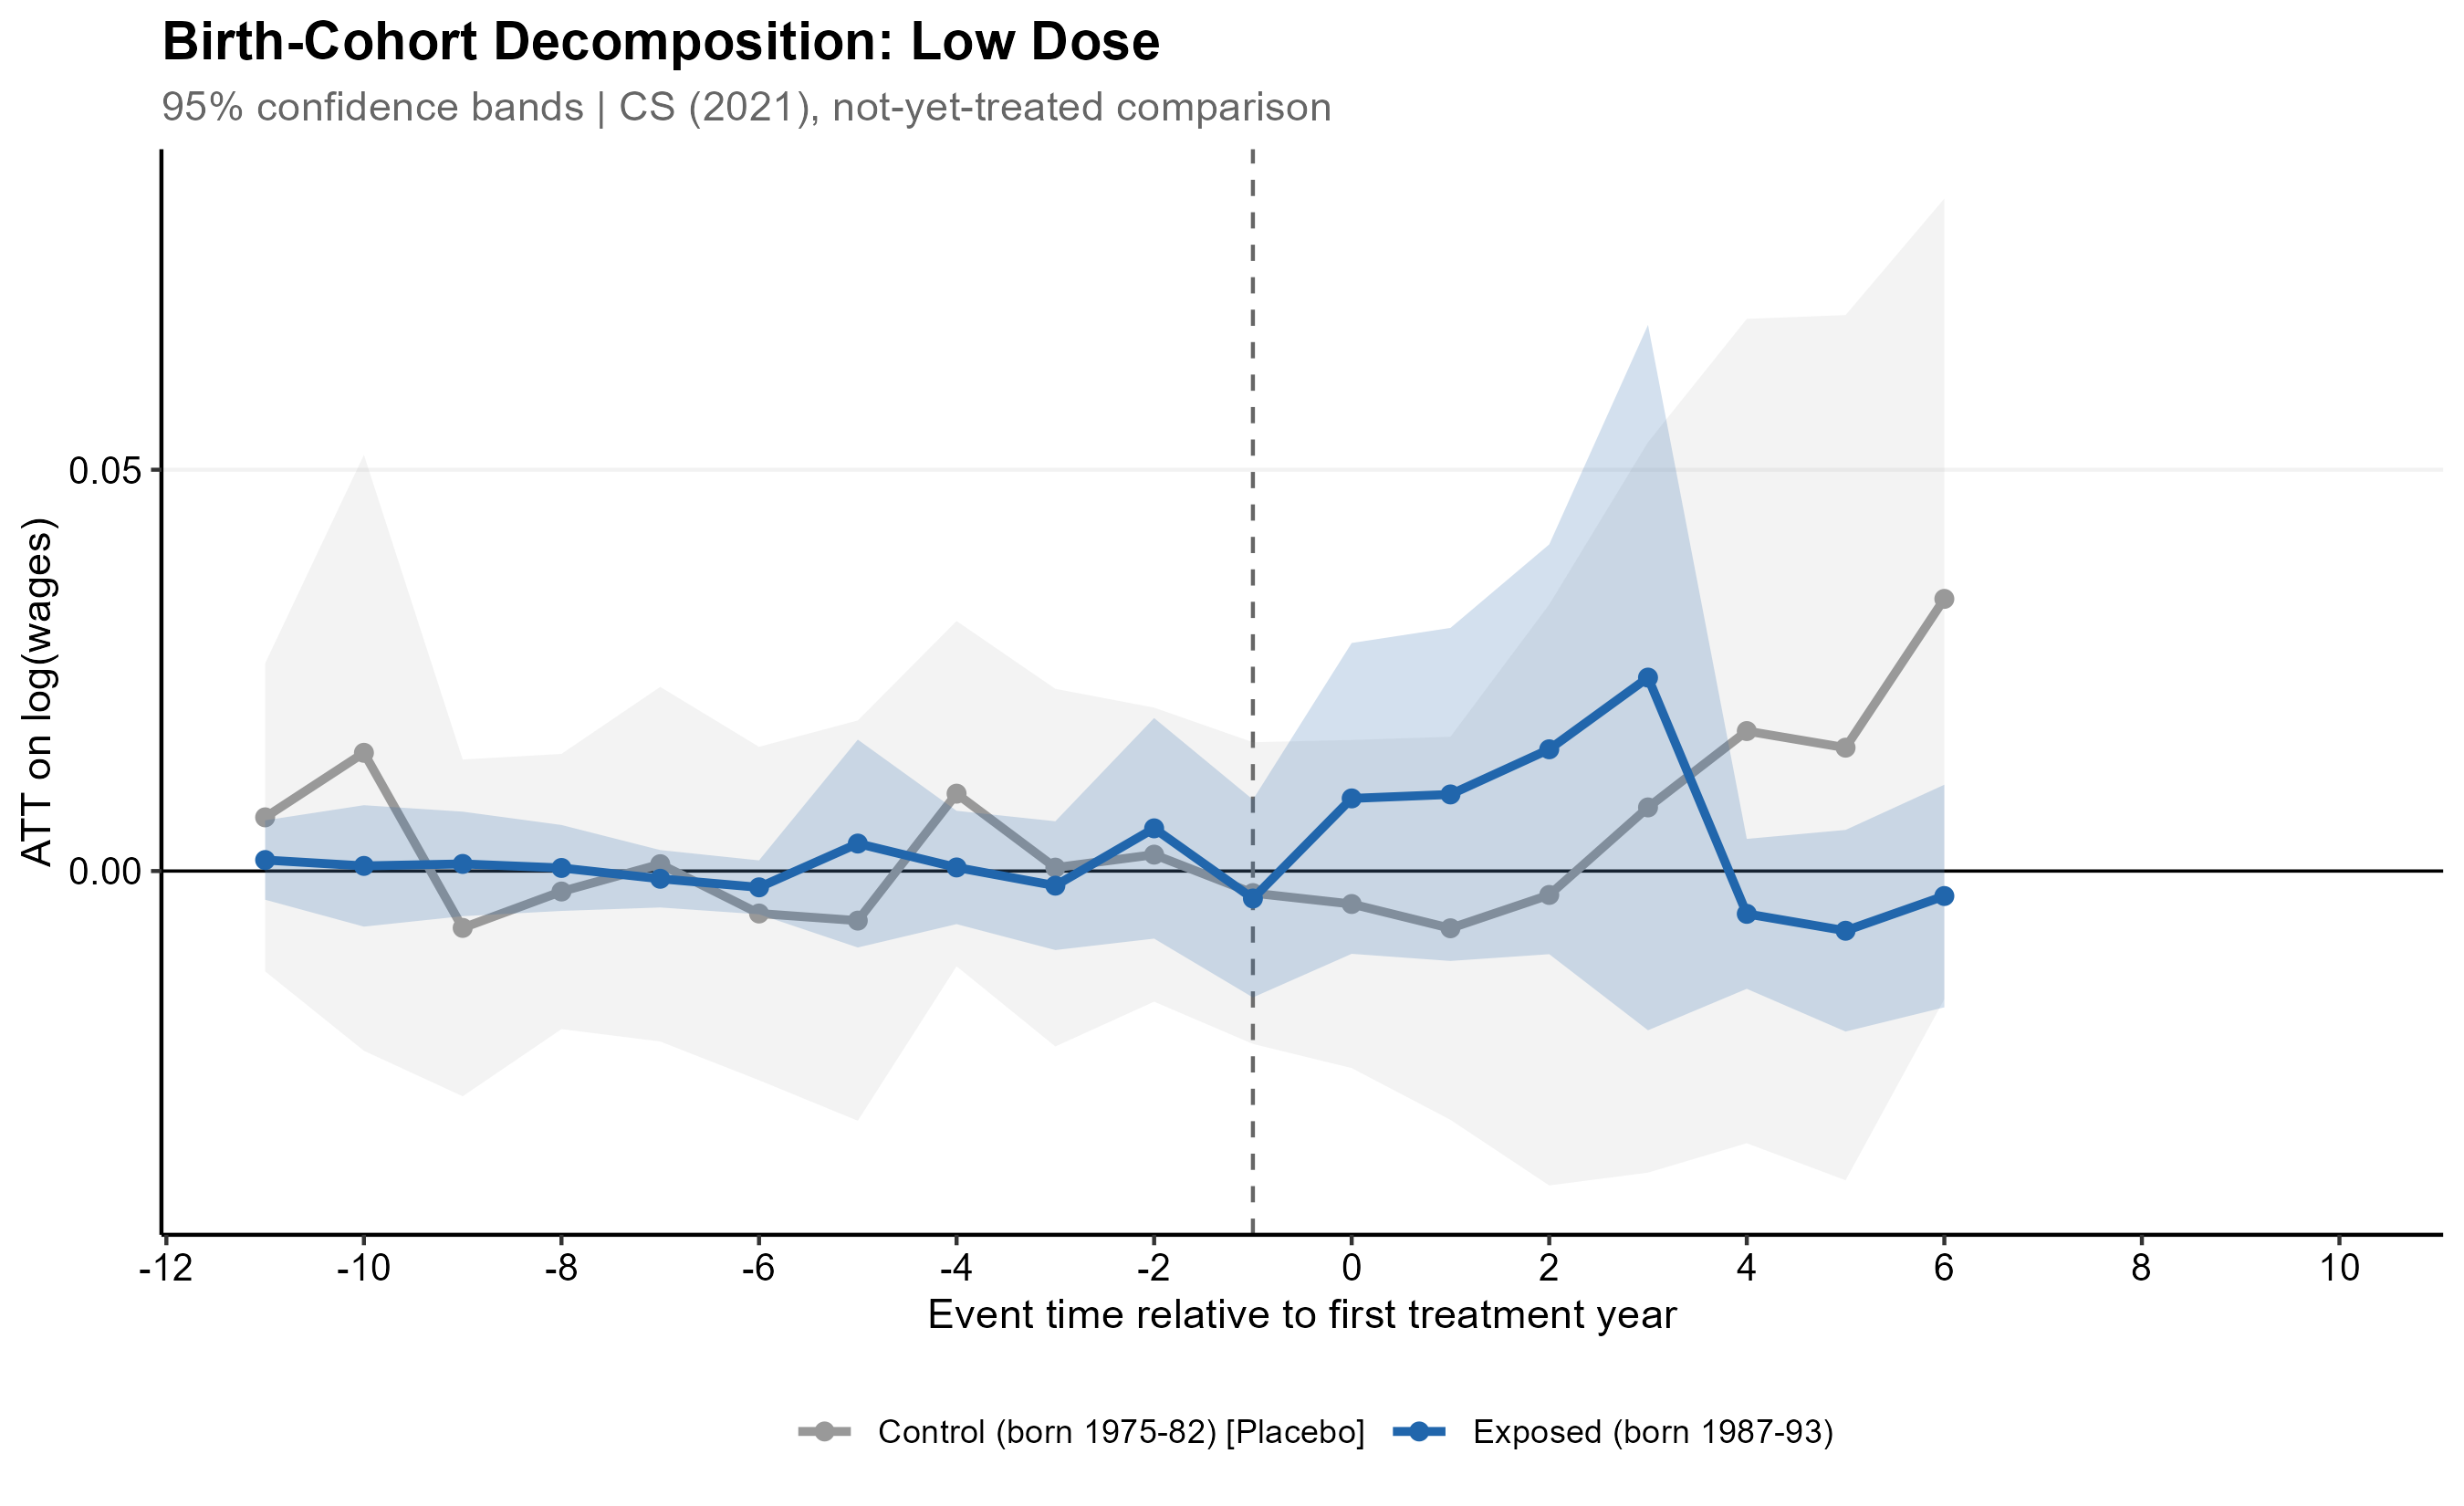
\includegraphics[width=0.84\textwidth]{Figures/fig_birthcohort_decomp.png}
    \caption{\textbf{Birth-cohort decomposition.} Supplementary decomposition of cohort-based wage dynamics.}
    \label{fig:app_birthcohort_decomp}
    \caption*{\footnotesize \textit{Notes:} This figure complements the main cohort-gap analysis by decomposing the dynamics into cohort-specific components. It is primarily useful for mechanism discussion rather than for establishing a separate headline treatment effect.}
\end{figure}

\begin{figure}[H]
    \centering
    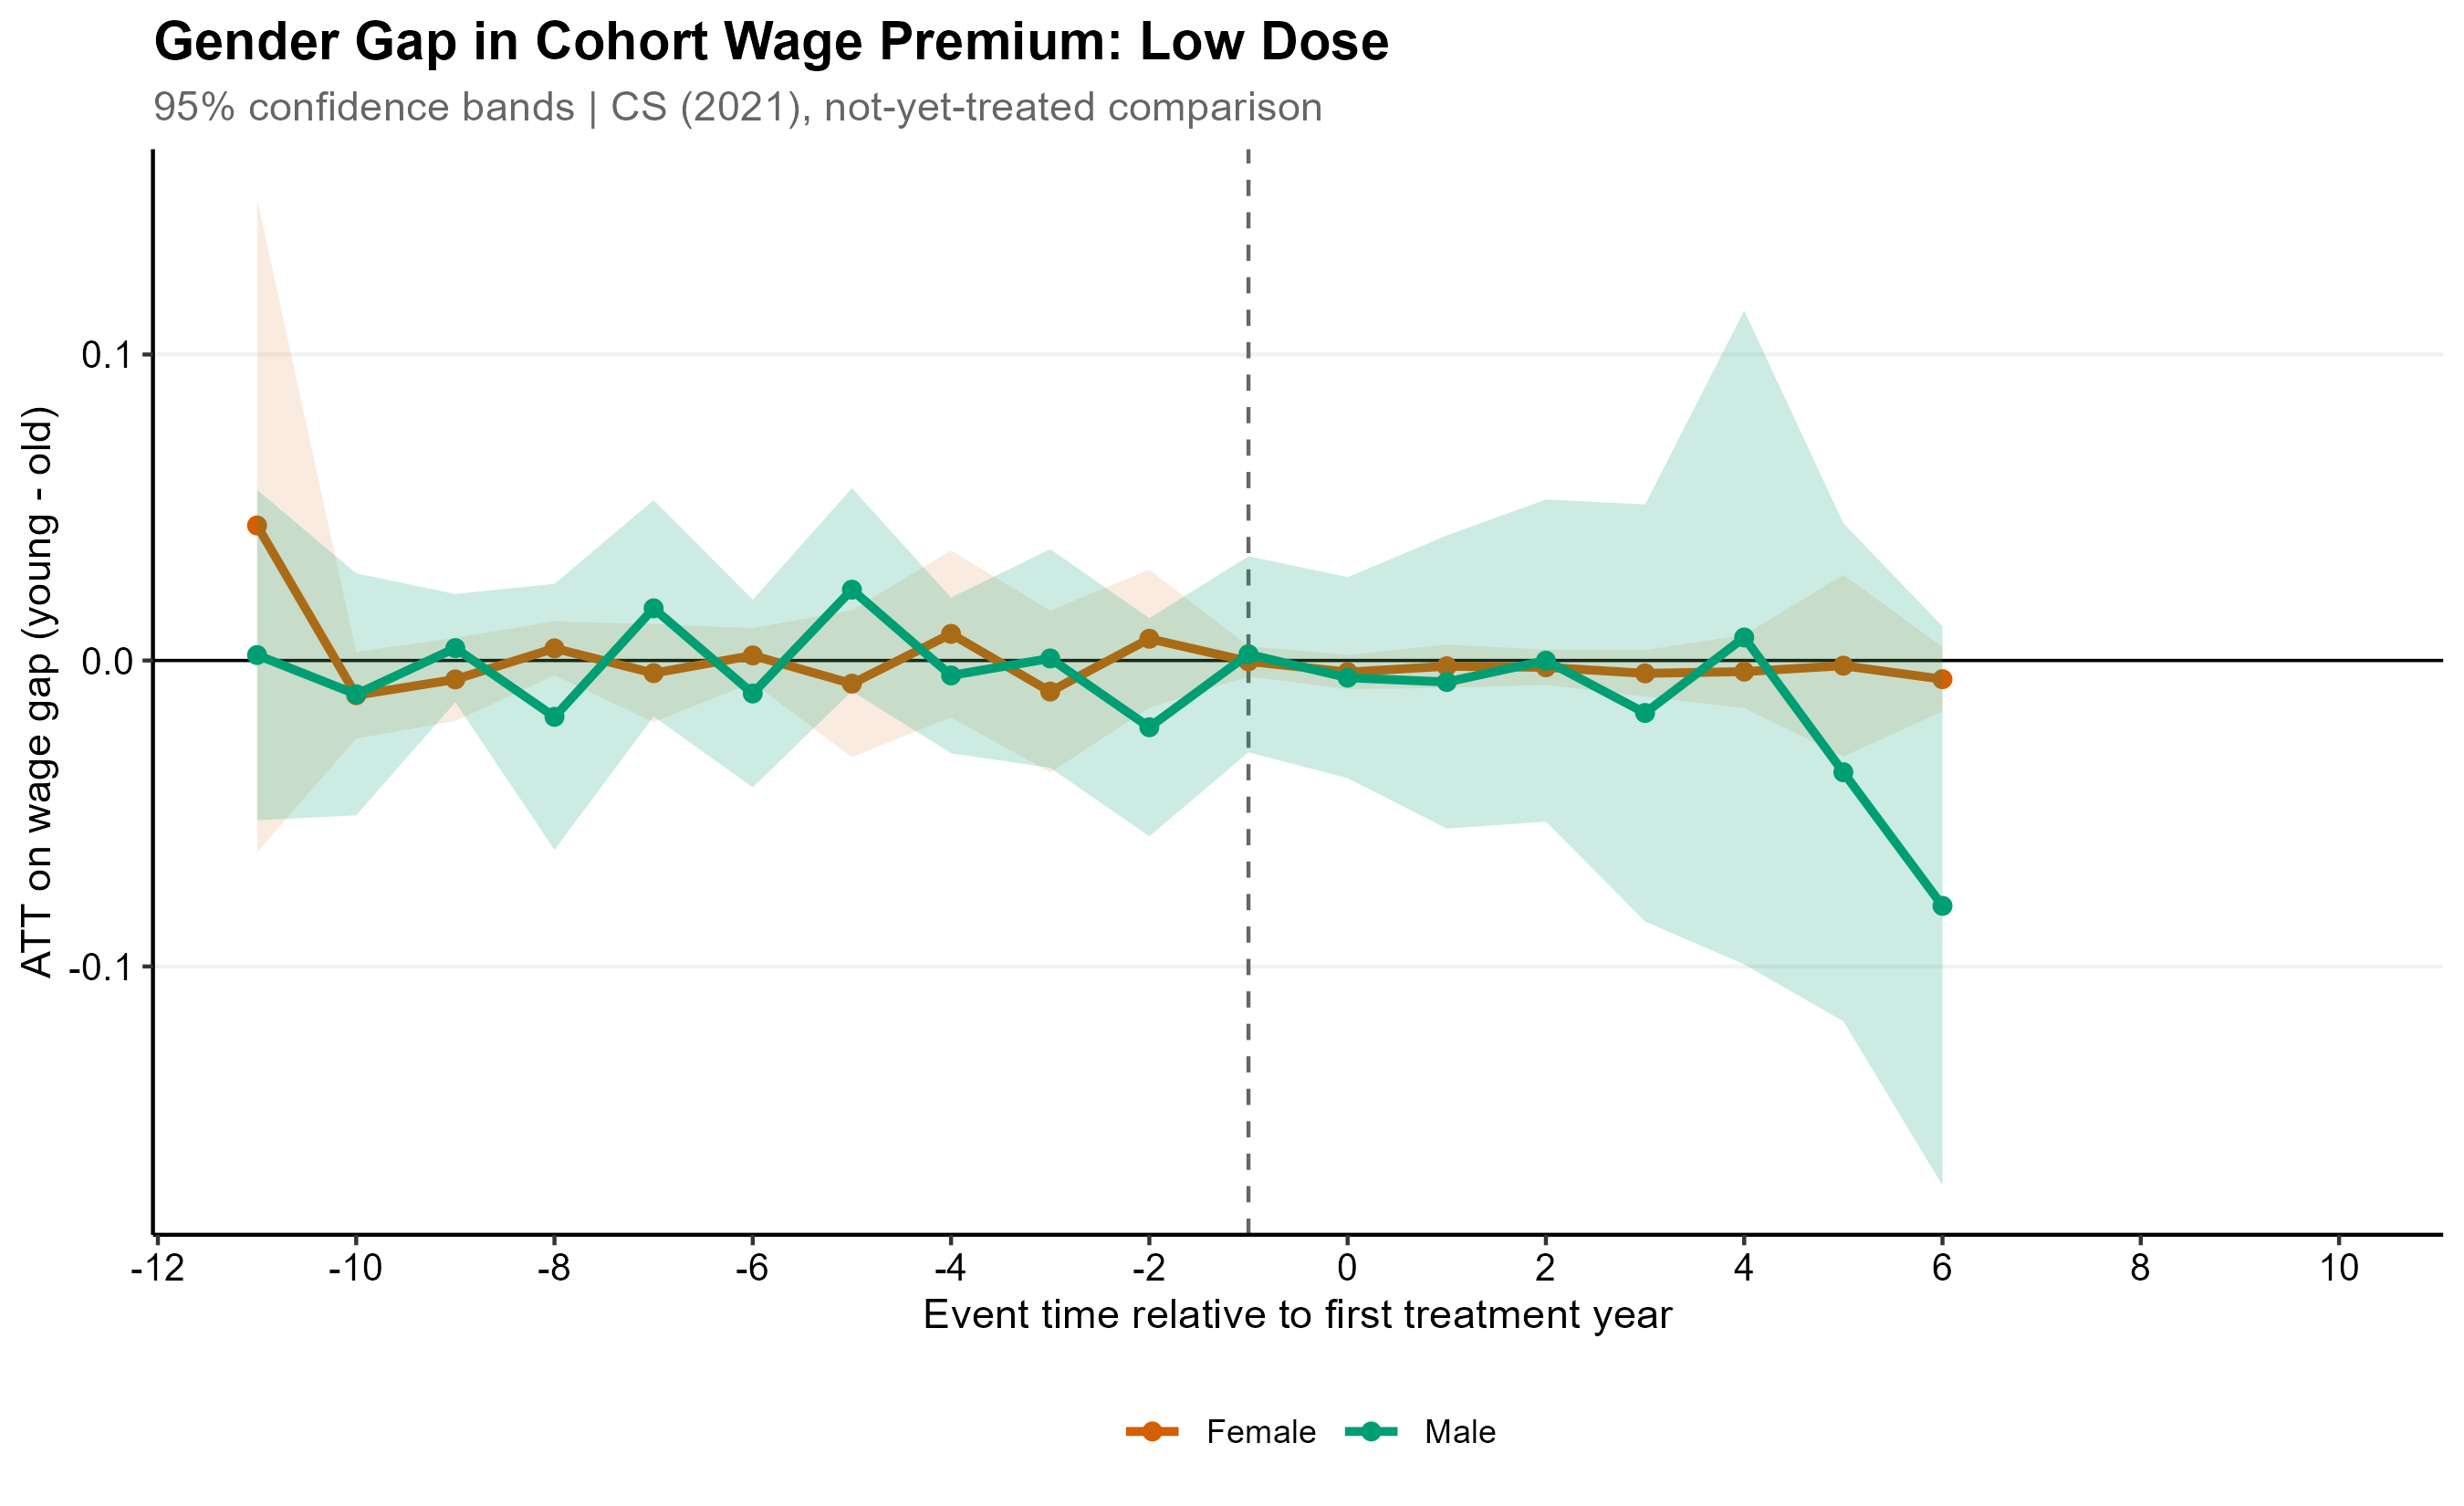
\includegraphics[width=0.49\textwidth]{Figures/fig_cohort_gender_low.png}
    \hfill
    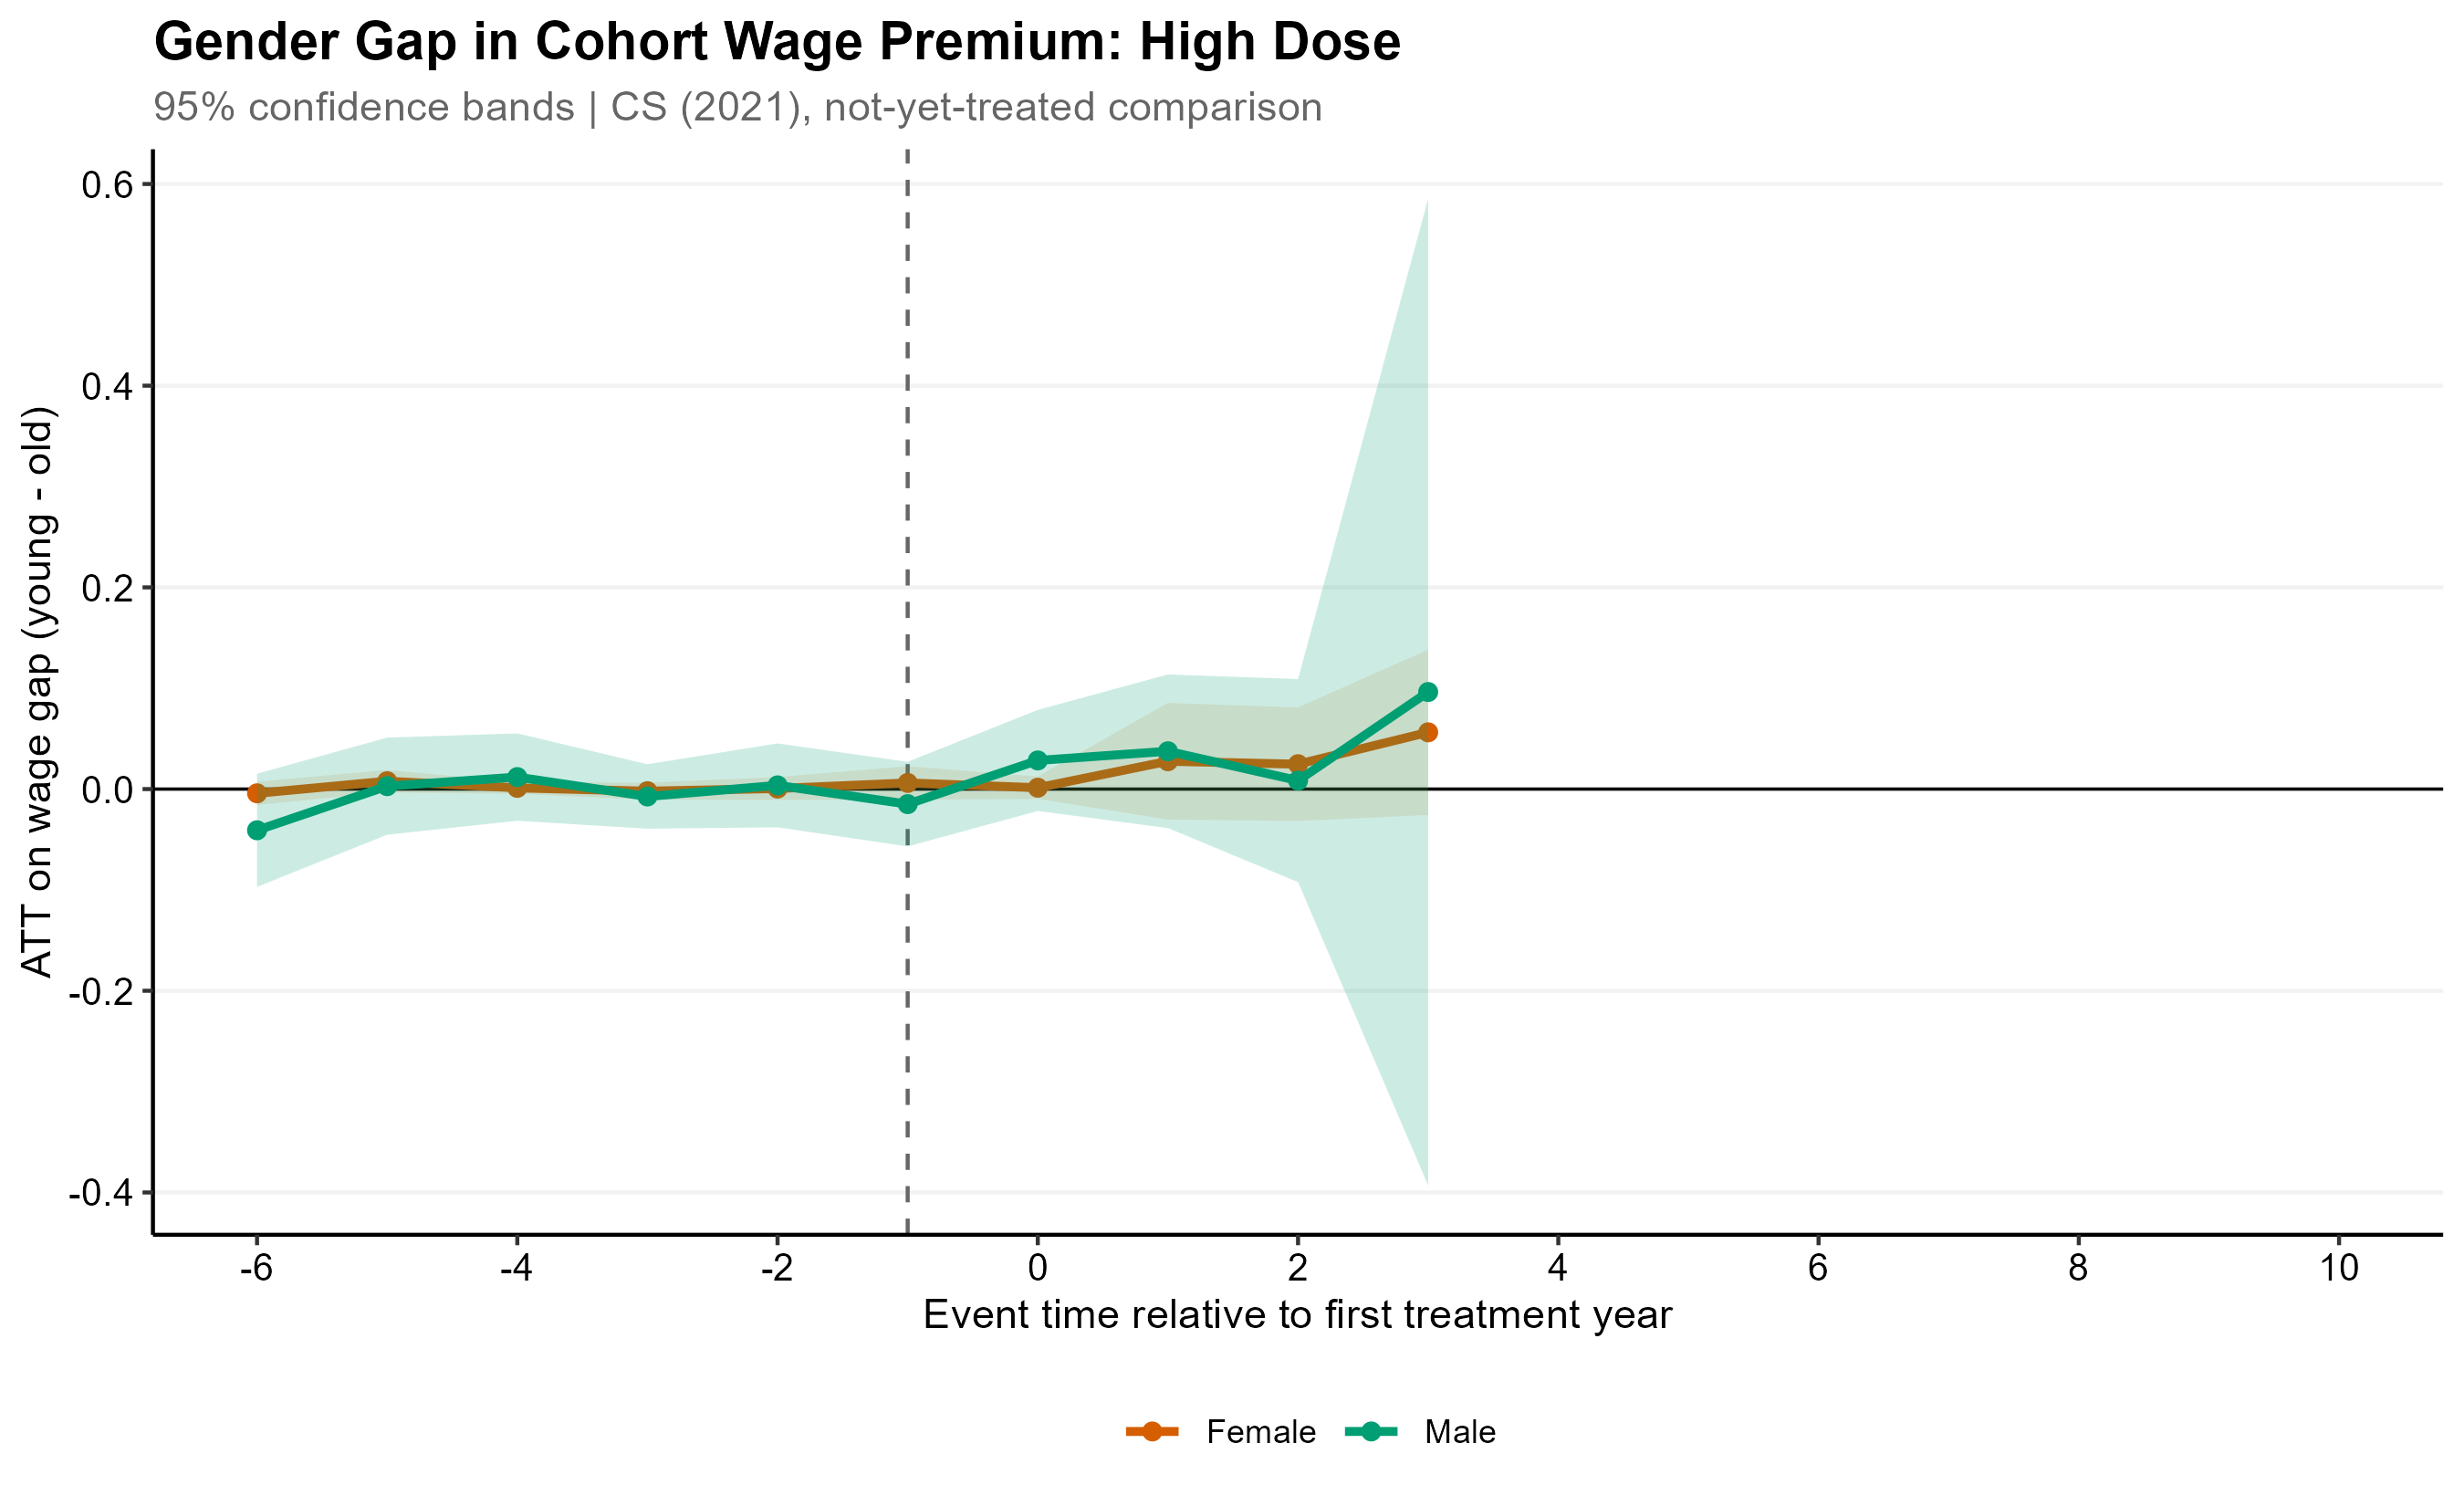
\includegraphics[width=0.49\textwidth]{Figures/fig_cohort_gender_high.png}
    \caption{\textbf{Cohort heterogeneity by gender.} Low-dose and high-dose cohort-gap estimates by gender.}
    \label{fig:app_cohort_gender}
    \caption*{\footnotesize \textit{Notes:} These subgroup estimates are included for completeness and to support the discussion of distributional incidence. As in the main text, they should be interpreted as reduced-form heterogeneity patterns rather than as evidence for a single structural mechanism.}
\end{figure}

\begin{figure}[H]
    \centering
    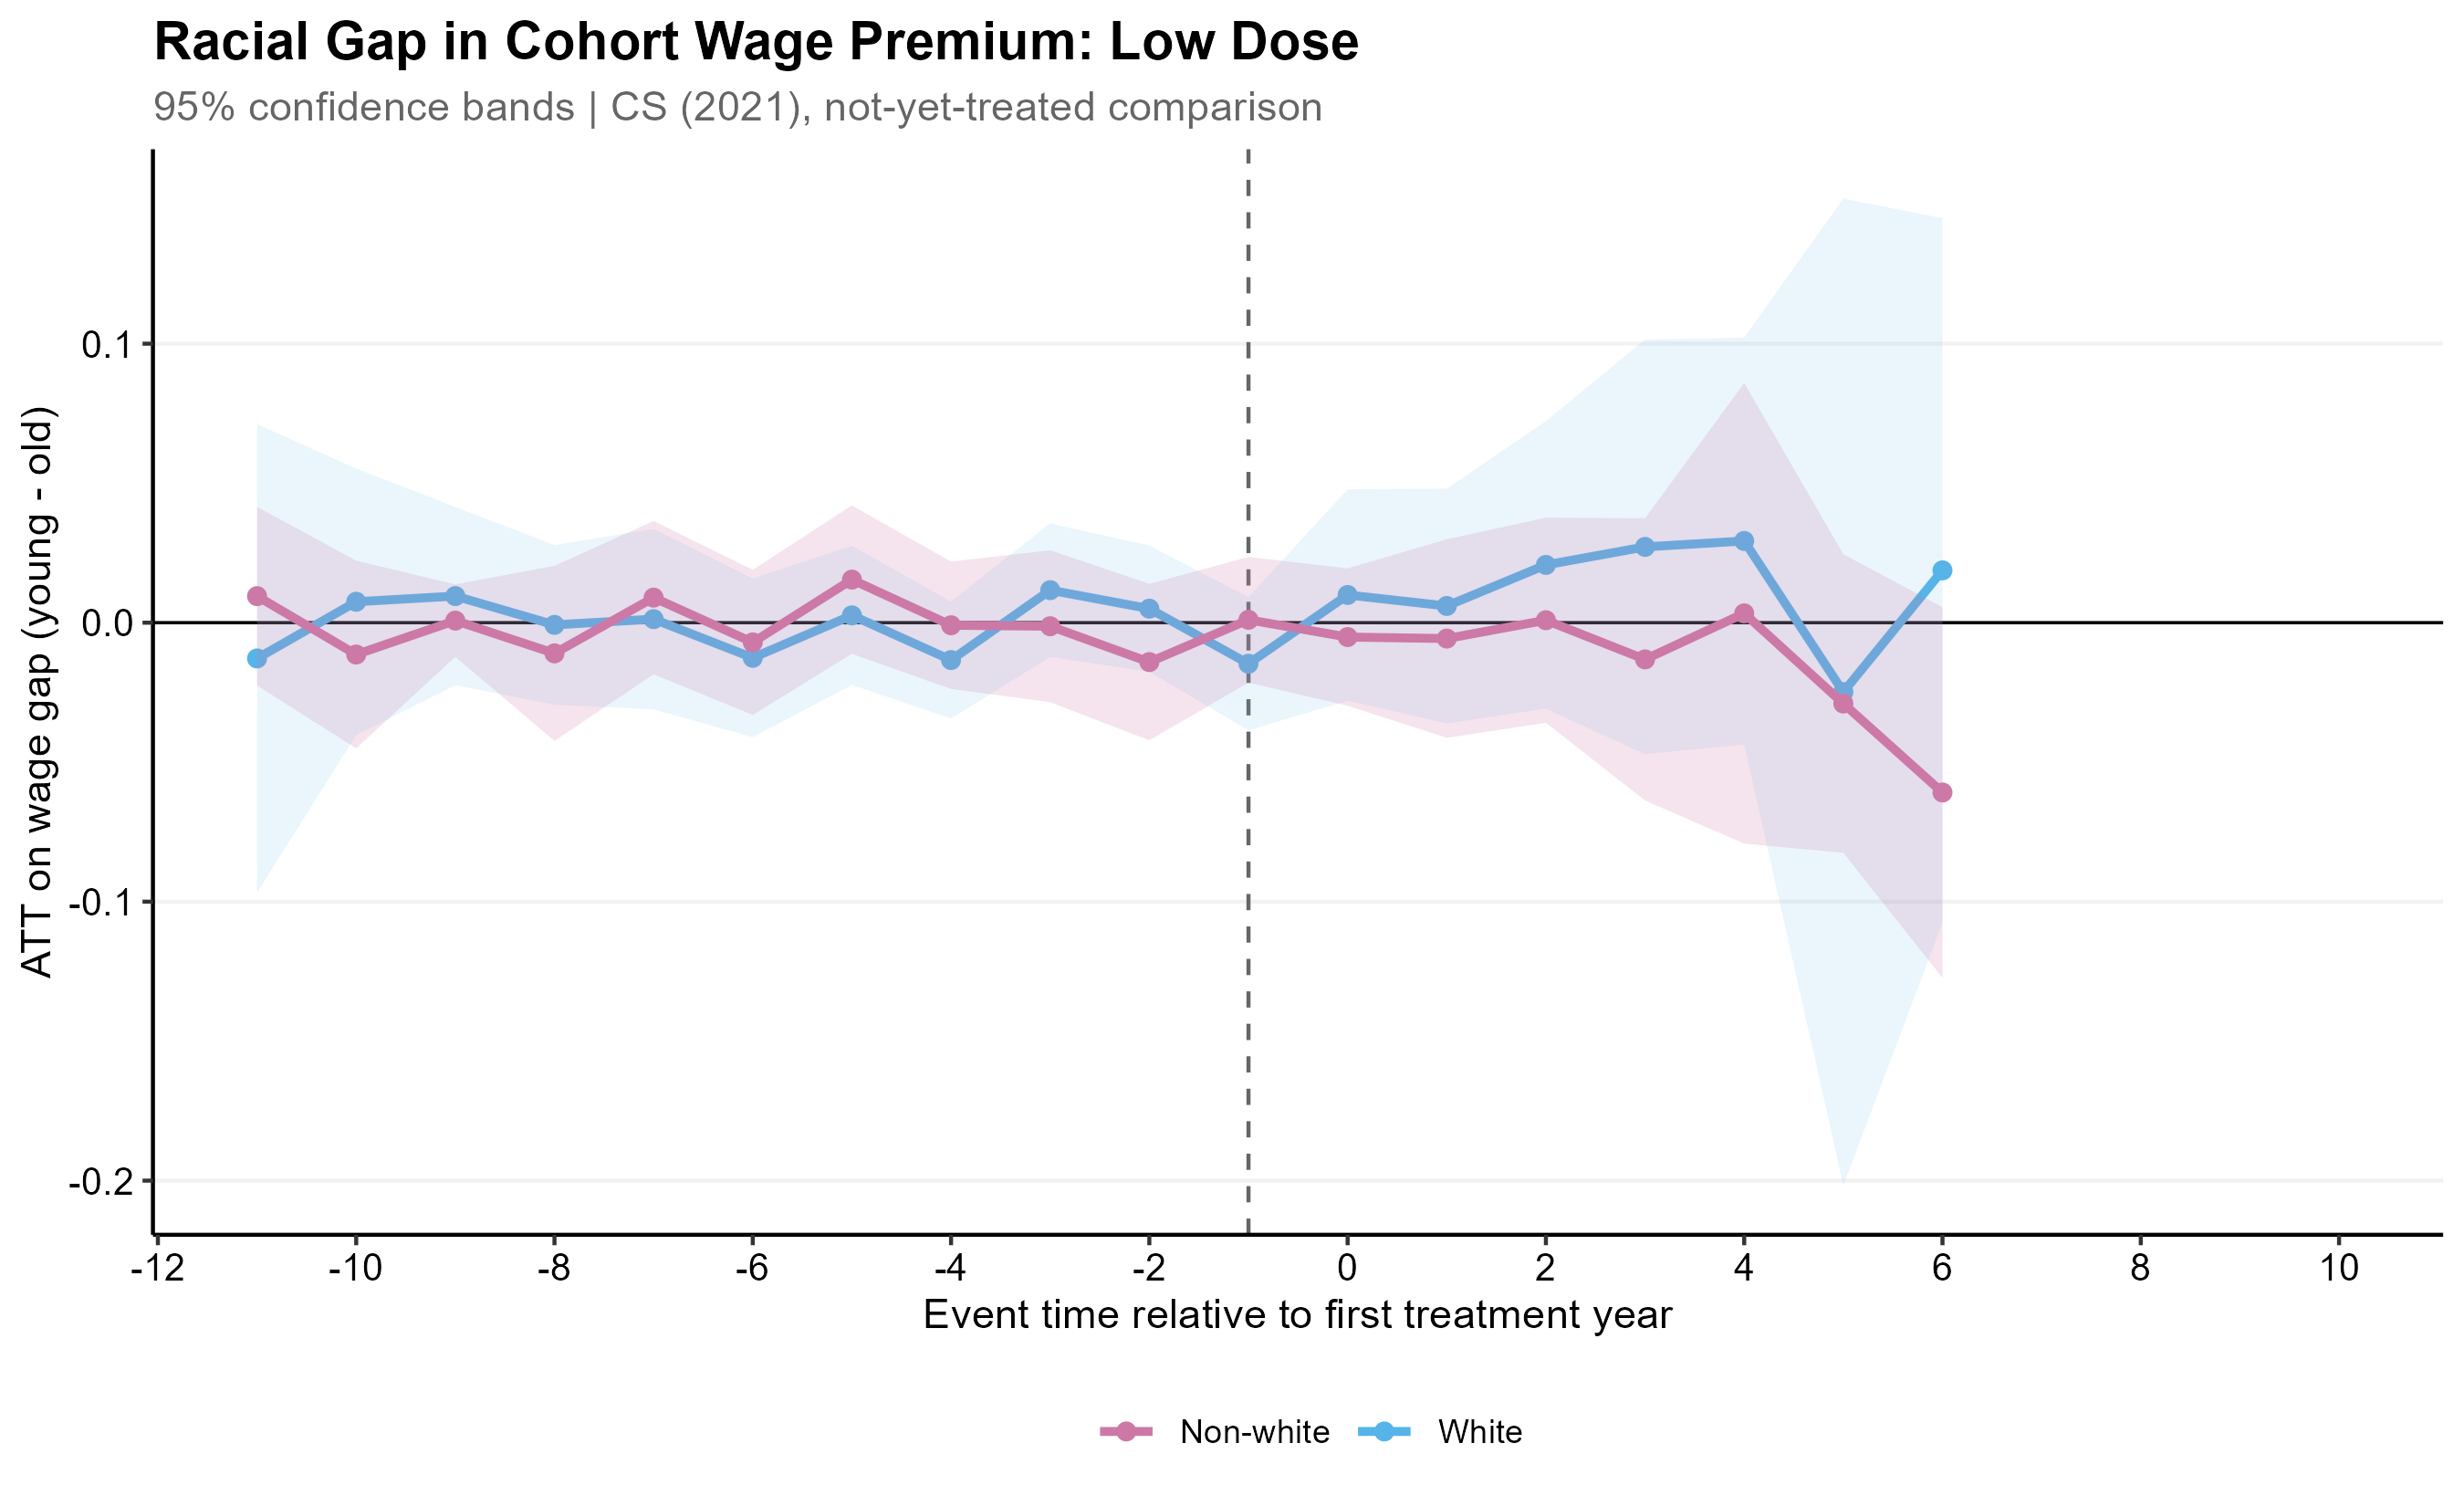
\includegraphics[width=0.49\textwidth]{Figures/fig_cohort_race_low.png}
    \hfill
    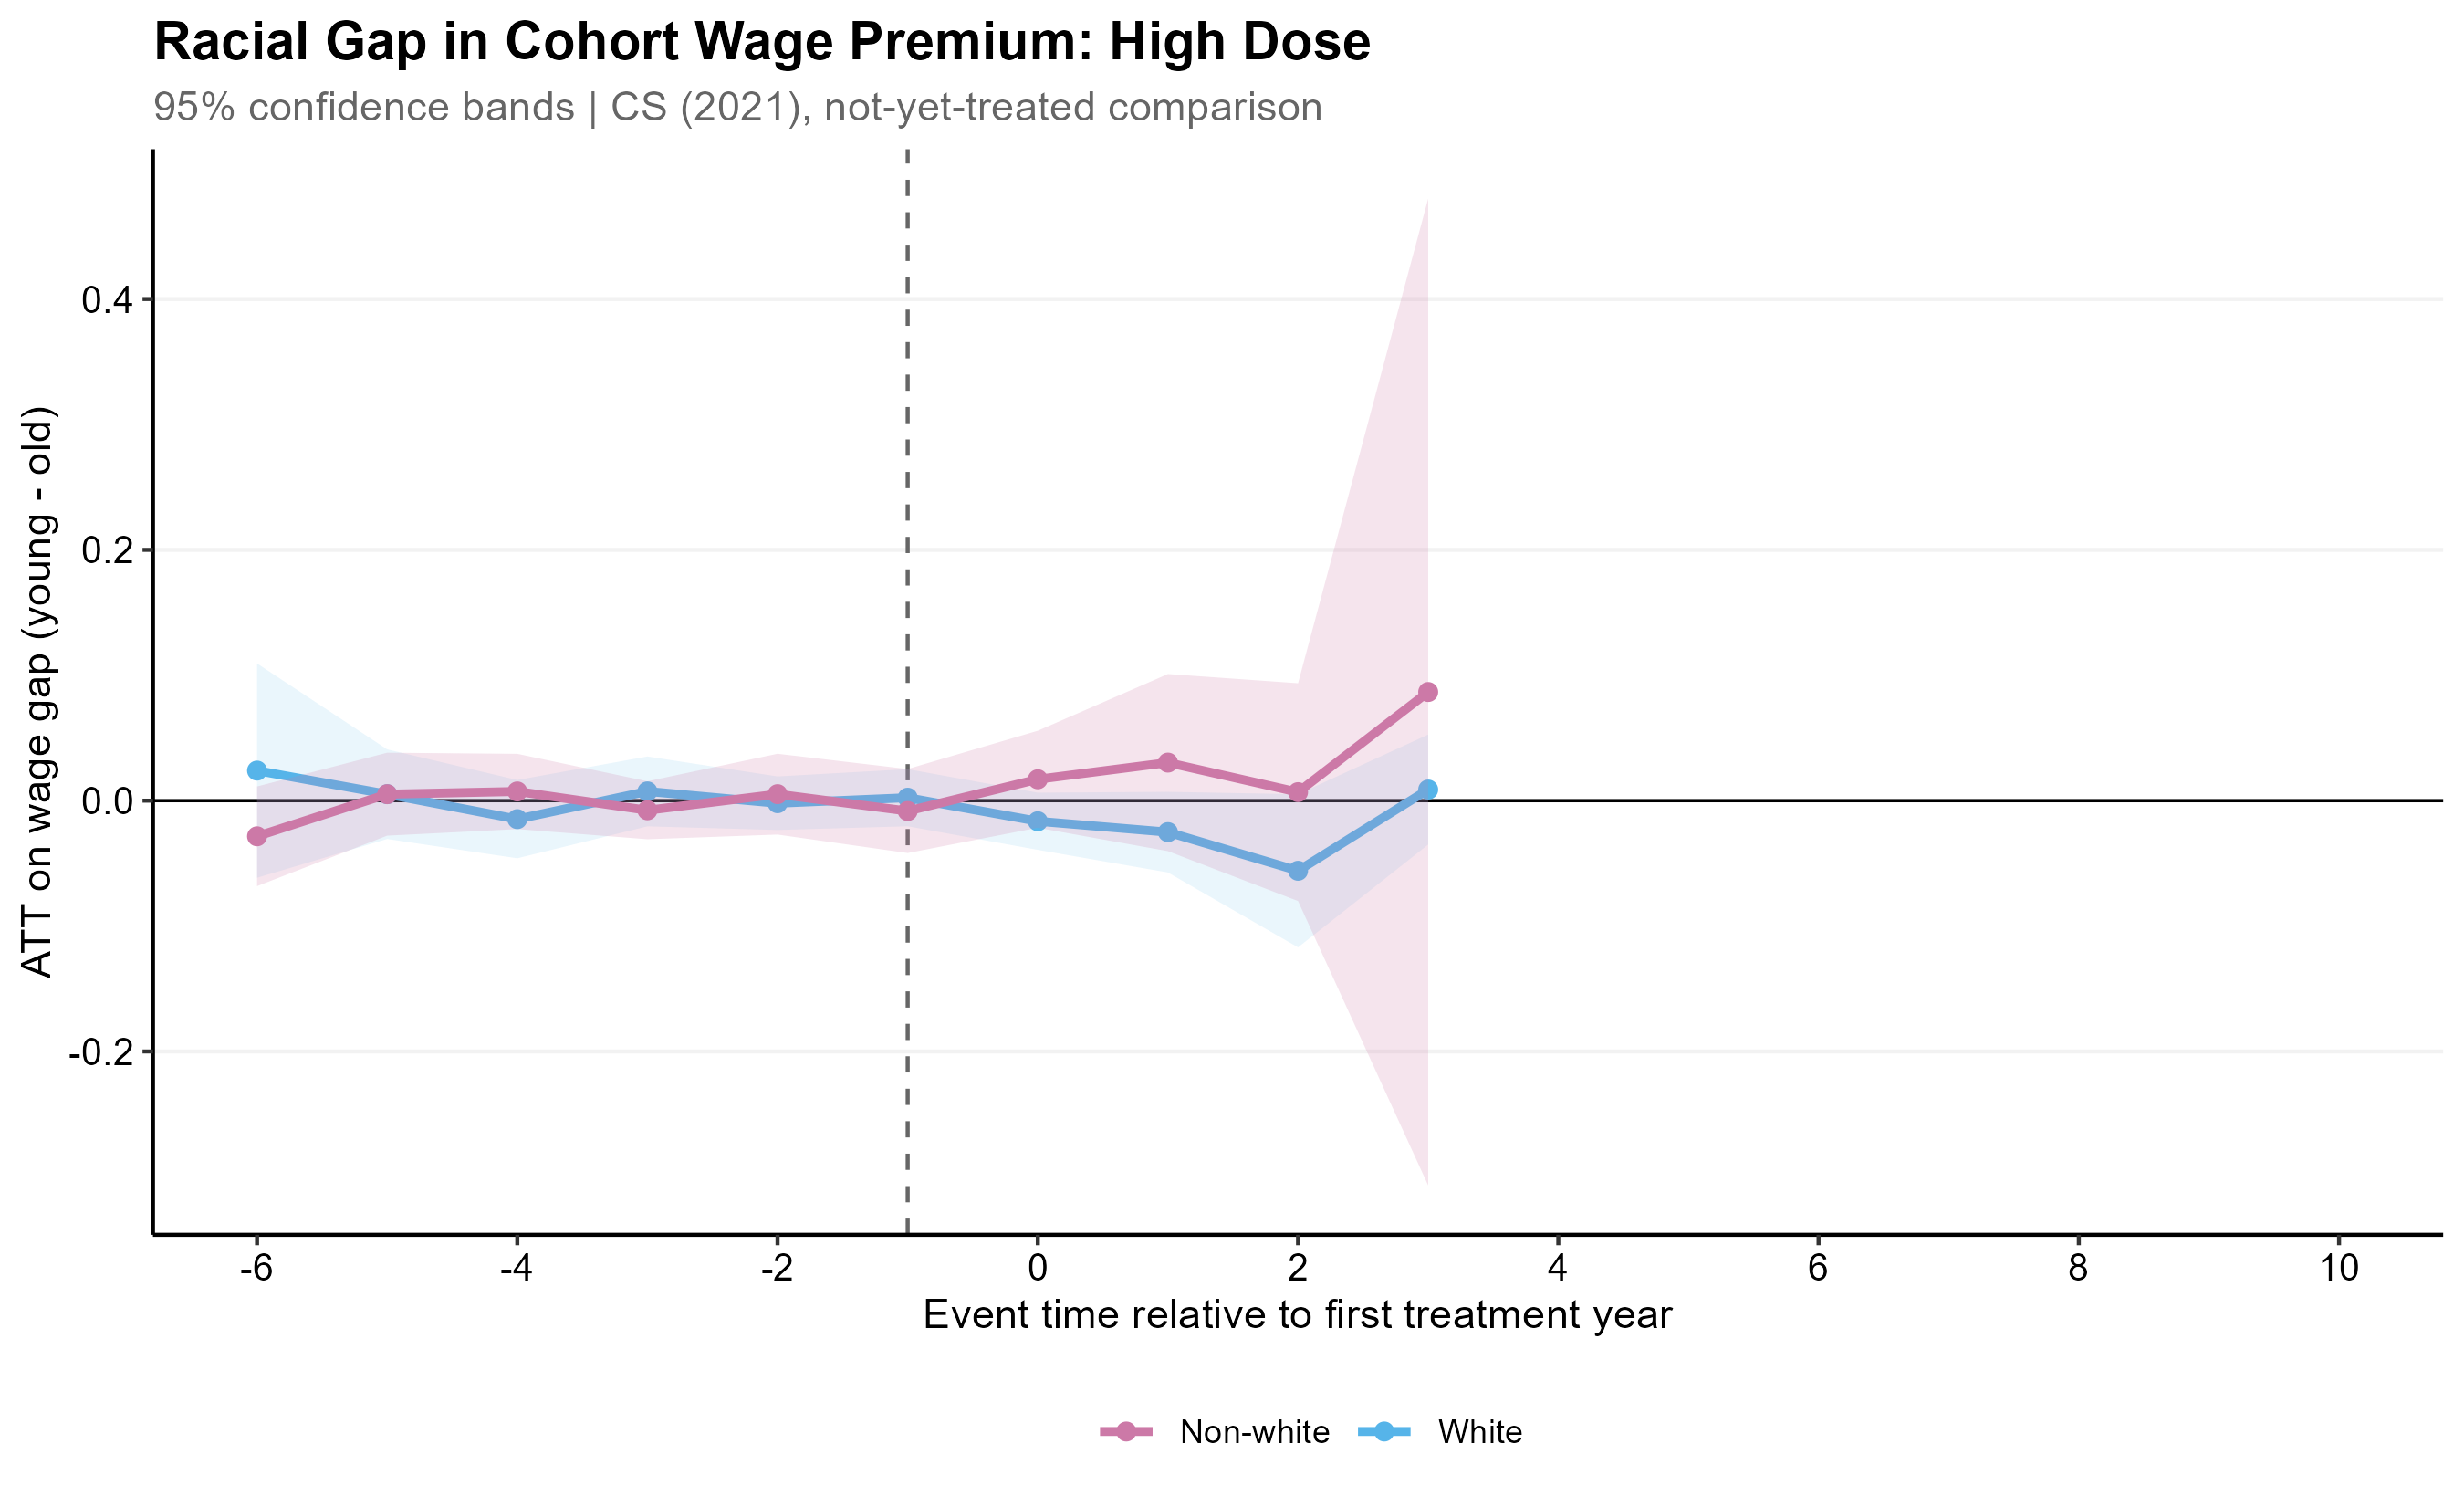
\includegraphics[width=0.49\textwidth]{Figures/fig_cohort_race_high.png}
    \caption{\textbf{Cohort heterogeneity by ethnicity.} Low-dose and high-dose cohort-gap estimates by ethnicity.}
    \label{fig:app_cohort_ethnicity}
    \caption*{\footnotesize \textit{Notes:} These figures provide supplementary evidence on whether the cohort-gap results differ across ethnicity groups. They are best interpreted as descriptive heterogeneity within the reduced-form framework adopted in the thesis.}
\end{figure}

% -----------------------------------------------------------------------
\subsection{Interpretation}
\label{app:appendix_interpretation}

Taken together, the supplementary material supports three conclusions. First, the baseline low-dose wage effect is not contradicted by the robustness exercises, but it is sensitive to treatment-intensity discretisation and lag choice. Second, the high-dose estimates remain weaker and do not provide decisive evidence for a clean saturation mechanism once broader specification uncertainty is acknowledged. Third, the cohort and subgroup exercises are informative about possible channels and distributional incidence, but they should not be treated as more credible than the primary pooled event-study evidence.
